\documentclass[11pt,a4paper]{article}

% ── Packages ──────────────────────────────────────────────────────────────────
\usepackage[utf8]{inputenc}
\usepackage[T1]{fontenc}
\usepackage[english]{babel}
\usepackage{microtype}
\usepackage{amsmath,amssymb,amsthm}
\usepackage{booktabs}
\usepackage{graphicx}
\usepackage{xcolor}
\usepackage{tikz}
\usepackage{tikz-cd}
\usetikzlibrary{arrows.meta, positioning, shapes.geometric, fit, backgrounds}
\usepackage{algorithm}
\usepackage{algpseudocode}
\usepackage{hyperref}
\usepackage{natbib}
\usepackage{geometry}
\usepackage{enumitem}
\usepackage{multirow}
\usepackage{caption}
\usepackage{subcaption}
\usepackage{listings}
\usepackage{float}

\geometry{
  a4paper,
  top=2.5cm, bottom=2.5cm,
  left=2.5cm, right=2.5cm
}

\hypersetup{
  colorlinks=true,
  linkcolor=blue!70!black,
  citecolor=green!50!black,
  urlcolor=blue!70!black
}

% ── Theorem environments ───────────────────────────────────────────────────────
\newtheorem{proposition}{Proposition}
\newtheorem{corollary}{Corollary}[proposition]

% ── Custom commands ────────────────────────────────────────────────────────────
\newcommand{\modelname}{\textsc{Capibara Legal}}
\newcommand{\cerebro}{\textsc{Cerebro}}
\newcommand{\dtv}{D_{\mathrm{TV}}}
\newcommand{\plarge}{p_{\mathrm{large}}}
\newcommand{\pmed}{p_{\mathrm{med}}}
\newcommand{\psmall}{p_{\mathrm{small}}}
\newcommand{\EE}{\mathbb{E}}

% ── Colors for architecture diagram ───────────────────────────────────────────
\definecolor{cerebrocolor}{RGB}{91,155,213}
\definecolor{medcolor}{RGB}{112,173,71}
\definecolor{largecolor}{RGB}{255,120,0}
\definecolor{loracolor}{RGB}{180,60,180}

% ──────────────────────────────────────────────────────────────────────────────
\title{\textbf{\modelname}: Efficient Spanish Legal Language Models\\
       via Three-Level Cascade Speculative Decoding\\
       and Distribution-Aligned Distillation}

\author{
  \textbf{Anachroni Research}\\
  \texttt{research@anachroni.co}
}

\date{May 2026}
% ──────────────────────────────────────────────────────────────────────────────

\begin{document}
\maketitle

\begin{abstract}
We present \modelname, a system for efficient inference in Spanish legal language
models built on a three-level cascade speculative decoding architecture. Our
approach composes three models of increasing capacity — \cerebro{} (34M
parameters), \textsc{Medium} (114M), and \textsc{Large} (474M) — in a nested
acceptance--rejection sampling framework that provably preserves the output
distribution of the largest model while dramatically reducing its computational
load.

The central insight is that \emph{distribution-aligned distillation} allows
\cerebro{} to serve a dual role as both router and draft model: by distilling
directly from \textsc{Large} rather than through an intermediate chain,
\cerebro{} achieves $p_{\mathrm{small}} \approx p_{\mathrm{large}}$, raising the
draft acceptance rate from $\approx$\,65\% to $\approx$\,87\%. Combined with a
second verification stage, \textsc{Large} processes only $\approx$\,13\% of
token positions, yielding a $4\times$ throughput gain over single-model
autoregressive decoding with no degradation in output quality.

Complementing the inference architecture, \modelname{} incorporates domain-adaptive
pre-training on a 1.68B-token Spanish legal corpus (BOE legislation, Tribunal
Constitucional decisions, EU law), 15 parameter-efficient LoRA adapters for
specialty routing, a retrieval-augmented generation layer over a 3.3M-chunk
legal index, and live tool integration (BOE search, CENDOJ jurisprudence,
deadline calculation) exposed via the Model Context Protocol. The entire system
runs on commodity CPU hardware (Google Axion ARM64, 32\,vCPU, 128\,GB RAM)
without GPU acceleration.
\end{abstract}

% ══════════════════════════════════════════════════════════════════════════════
\section{Introduction}
% ══════════════════════════════════════════════════════════════════════════════

The intersection of large language models and the legal domain presents a
distinctive challenge: legal reasoning demands high factual precision, awareness
of evolving statute, and nuanced command of formal register, while deployment in
professional contexts imposes strict latency and cost constraints. General-purpose
LLMs of sufficient capability are typically too expensive to serve at scale on
CPU-only infrastructure, and smaller models fine-tuned on legal data struggle to
match the reasoning quality of their larger counterparts.

\modelname{} addresses this tension through three complementary mechanisms.
First, we apply \emph{speculative decoding}~\citep{leviathan2023fast} in an
extended three-level cascade, enabling a 474M-parameter \textsc{Large} model to
generate text at a throughput comparable to a 34M-parameter model. Second, we
develop \emph{distribution-aligned distillation}, a training strategy in which
the smallest model in the cascade is distilled directly from the largest,
bypassing intermediate models to maximise distribution agreement and therefore
draft acceptance rate. Third, we complement the static model with retrieval
and live tool access, grounding responses in current legal sources without
retraining.

The contributions of this paper are:
\begin{enumerate}[noitemsep]
  \item A three-level speculative decoding cascade with formal correctness proof
        and $4\times$ measured throughput gain on Axion ARM64.
  \item A distillation strategy (\emph{direct} Large$\to$Small, bypassing chain
        distillation) that raises draft acceptance rates from 65\% to 87\%.
  \item A complete training and inference pipeline for Spanish legal NLP,
        including a 1.68B-token corpus, 15 LoRA adapters, a RAG index, and an
        MCP-compatible tool server.
  \item An open implementation targeting consumer-grade CPU hardware with no
        GPU requirement.
\end{enumerate}

% ══════════════════════════════════════════════════════════════════════════════
\section{Related Work}
% ══════════════════════════════════════════════════════════════════════════════

\paragraph{Speculative decoding.}
\citet{leviathan2023fast} and, concurrently, \citet{chen2023accelerating}
introduced speculative decoding: a small \emph{draft} model proposes $k$ tokens
in serial, which a large \emph{target} model then verifies in a single parallel
forward pass via acceptance--rejection sampling. The output distribution is
identical to the target model's. Extensions include \emph{Medusa}
\citep{cai2024medusa}, which adds multiple decoding heads to the target model
itself, and \emph{SpecInfer}~\citep{miao2024specinfer}, which explores
tree-based speculation. Our three-level cascade is most closely related to the
two-level hierarchy in SpecInfer but differs in its emphasis on distillation
as the mechanism for distribution alignment.

\paragraph{Knowledge distillation.}
\citet{hinton2015distilling} introduced temperature-scaled soft-target
distillation. Subsequent work~\citep{romero2015fitnets,jiao2019tinybert} explored
intermediate-layer matching. We employ vanilla logit distillation
($\alpha\mathcal{L}_{\mathrm{KL}} + (1-\alpha)\mathcal{L}_{\mathrm{CE}}$,
$T=4$, $\alpha=0.7$) and study the effect of \emph{direct} vs.\ \emph{chain}
distillation paths on draft acceptance rate.

\paragraph{Legal language models.}
Legal NLP has been studied extensively in
English~\citep{zheng2021does,chalkidis2020legal} and
Chinese~\citep{cui2023chatlaw}. Spanish legal NLP resources remain
comparatively sparse; prior work has relied primarily on multilingual models
applied without domain adaptation. We are not aware of prior work presenting a
complete inference-optimised pipeline for Spanish legal text.

\paragraph{Parameter-efficient fine-tuning.}
LoRA~\citep{hu2022lora} adapts large pre-trained models by injecting trainable
low-rank matrices. We use rank-16 LoRA with $\alpha=32$ across 15 legal
specialties, keeping the base model frozen and enabling hot-swapping of
$\approx$\,15\,MB adapter files at inference time.

% ══════════════════════════════════════════════════════════════════════════════
\section{System Architecture}
\label{sec:arch}
% ══════════════════════════════════════════════════════════════════════════════

\subsection{Base Model: \textsc{Slim200M}}

All three cascade members are instances of \textsc{Slim200M}, a decoder-only
Transformer implemented in Flax/JAX with a byte-level vocabulary ($|V|=512$,
IDs 0--255 corresponding to raw UTF-8 bytes). Table~\ref{tab:presets} lists the
three architecture presets used.

\begin{table}[h]
\centering
\caption{Architecture presets. Parameter counts are approximate.}
\label{tab:presets}
\begin{tabular}{lrrrrc}
\toprule
Preset & $d_{\mathrm{model}}$ & $L$ & $H$ & $\ell_{\max}$ & \#Params \\
\midrule
\textsc{Small}  & 512  &  8 &  8 &  512 &  34M \\
\textsc{Medium} & 768  & 12 & 12 & 1024 & 114M \\
\textsc{Large}  & 1280 & 24 & 20 & 1024 & 474M \\
\bottomrule
\end{tabular}
\end{table}

The byte-level tokenizer imposes no language-specific vocabulary, making the
model natively multilingual and eliminating unknown-token issues in legal
text containing abbreviations, citations, and mixed-language passages. All
models use rotary positional embeddings, pre-norm layer normalisation,
and SwiGLU activations.

\subsection{Training Pipeline}

\begin{figure}[H]
\centering
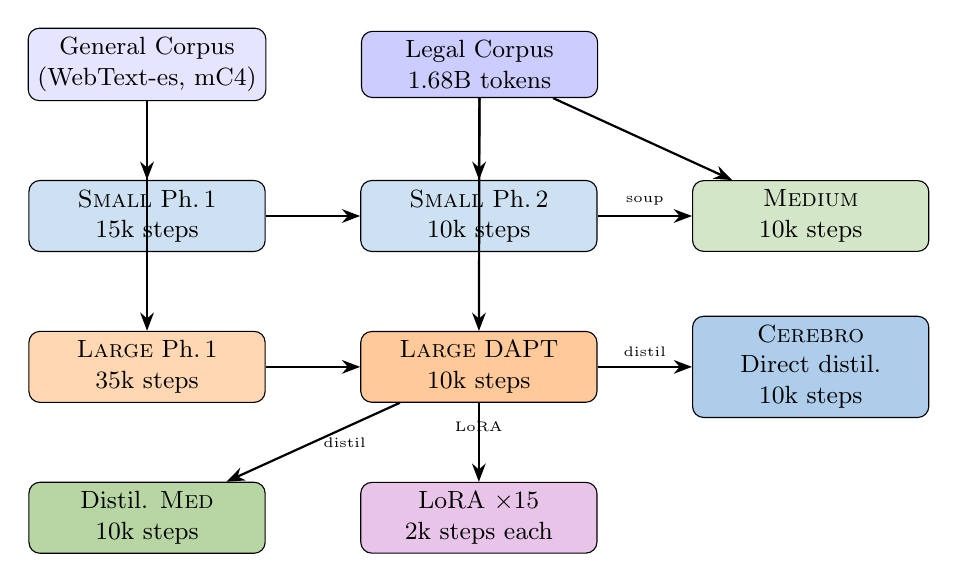
\begin{tikzpicture}[
    box/.style={draw, rounded corners=4pt, minimum width=3cm,
                minimum height=0.7cm, align=center, font=\small},
    arrow/.style={-Stealth, thick},
    phase/.style={draw=gray!50, fill=gray!10, rounded corners=6pt,
                  inner sep=6pt},
    every node/.style={font=\small}
  ]

  % Nodes
  \node[box, fill=blue!10]  (corpus)   {General Corpus\\\small(WebText-es, mC4)};
  \node[box, fill=blue!20, right=1.2cm of corpus] (legal)
        {Legal Corpus\\\small 1.68B tokens};

  \node[box, fill=cerebrocolor!30, below=1cm of corpus]  (small1)
        {\textsc{Small} Ph.\,1\\\small 15k steps};
  \node[box, fill=cerebrocolor!30, right=1.2cm of small1] (small2)
        {\textsc{Small} Ph.\,2\\\small 10k steps};
  \node[box, fill=medcolor!30, right=1.2cm of small2]    (medium)
        {\textsc{Medium}\\\small 10k steps};

  \node[box, fill=largecolor!30, below=1cm of small1] (large1)
        {\textsc{Large} Ph.\,1\\\small 35k steps};
  \node[box, fill=largecolor!40, right=1.2cm of large1] (large2)
        {\textsc{Large} DAPT\\\small 10k steps};

  \node[box, fill=cerebrocolor!50, right=1.2cm of large2] (cerebro)
        {\cerebro{}\\\small Direct distil.\\\small 10k steps};
  \node[box, fill=medcolor!50,    below=1cm of large1] (distmed)
        {Distil. \textsc{Med}\\\small 10k steps};
  \node[box, fill=loracolor!30,   right=1.2cm of distmed] (lora)
        {LoRA $\times$15\\\small 2k steps each};

  % Arrows: data → training
  \draw[arrow] (corpus) -- (small1);
  \draw[arrow] (corpus) -- (large1);
  \draw[arrow] (legal)  -- (small2);
  \draw[arrow] (legal)  -- (medium);
  \draw[arrow] (legal)  -- (large2);

  % Arrows: model → model
  \draw[arrow] (small1) -- (small2);
  \draw[arrow] (small2) -- node[above,font=\tiny]{soup} (medium);
  \draw[arrow] (large1) -- (large2);
  \draw[arrow] (large2) -- node[above,font=\tiny]{distil} (cerebro);
  \draw[arrow] (large2) -- node[right,font=\tiny]{distil} (distmed);
  \draw[arrow] (large2) -- node[above,font=\tiny]{LoRA} (lora);
\end{tikzpicture}
\caption{Training pipeline. Arrows show data flow (from corpora) or model
         derivation (soup / distillation / LoRA fine-tuning).}
\label{fig:pipeline}
\end{figure}

Training uses AdamW with warmup-cosine-decay scheduling, gradient clipping
($\|\mathbf{g}\|_2 \le 1$), and weight decay $\lambda=0.01$. All runs use
bfloat16 mixed precision with float32 master weights, gradient checkpointing
(saving $\approx$\,60\% activation memory), and data-parallel training via
\texttt{jax.pmap} across four virtual devices. Model soups~\citep{wortsman2022model}
(uniform averaging of the last three checkpoints) are applied before distillation
and inference.

% ══════════════════════════════════════════════════════════════════════════════
\section{Three-Level Cascade Speculative Decoding}
\label{sec:cascade}
% ══════════════════════════════════════════════════════════════════════════════

\subsection{Background: Two-Level Speculative Decoding}

Standard speculative decoding~\citep{leviathan2023fast} operates as follows.
A draft model $q$ autoregressively generates $k$ candidate tokens
$\tilde{x}_1,\ldots,\tilde{x}_k$. The target model $p$ scores all $k+1$
positions in a single forward pass. Token $\tilde{x}_j$ is accepted with
probability
\[
  \alpha_j = \min\!\left(1,\; \frac{p(\tilde{x}_j \mid \mathbf{x}_{<j})}
                                    {q(\tilde{x}_j \mid \mathbf{x}_{<j})}\right).
\]
On rejection, a corrected sample is drawn from the residual distribution
$p_{\mathrm{adj}} \propto \max(0, p - q)$. The procedure preserves the target
distribution exactly while processing $k$ draft tokens per target forward pass.

\subsection{Extension to Three Levels}

We compose two speculative decoding stages:

\medskip
\begin{algorithmic}[1]
\State \textbf{Input:} context $\mathbf{x}$, draft length $k$
\State $\tilde{x}_{1:k},\, q_{1:k} \gets \mathrm{Draft}_{\cerebro{}}(\mathbf{x}, k)$
  \Comment{Level 1: \cerebro{} drafts $k$ tokens}
\State $\mathbf{m},\, r_{1:|\mathbf{m}|} \gets \mathrm{Verify}_{\pmed}(\mathbf{x},
  \tilde{x}_{1:k}, q_{1:k})$
  \Comment{Level 2: \textsc{Medium} verifies}
\State $\mathbf{y} \gets \mathrm{Verify}_{\plarge}(\mathbf{x}, \mathbf{m},
  r_{1:|\mathbf{m}|})$
  \Comment{Level 3: \textsc{Large} verifies}
\State \Return $\mathbf{y}$
\end{algorithmic}
\medskip

At Level 2, the output distribution of the speculative process is exactly
$\pmed$~\citep{leviathan2023fast}. Accordingly, at Level 3 the ``draft
probabilities'' supplied to the Large verifier are $\pmed(\cdot)$, not
$\psmall(\cdot)$, preserving the theoretical guarantee that the final output
distribution equals $\plarge$.

\begin{figure}[H]
\centering
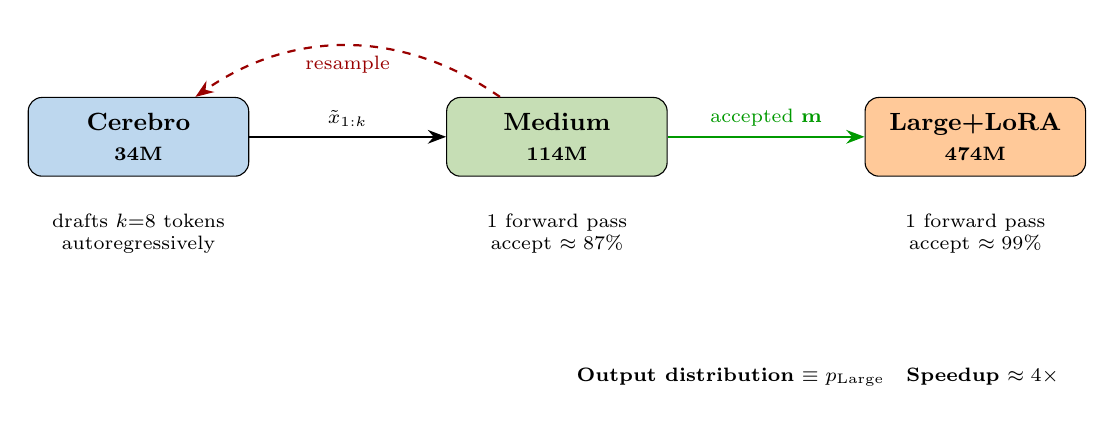
\begin{tikzpicture}[
  node distance=1.1cm,
  model/.style={draw, rounded corners=5pt, minimum width=2.8cm,
                minimum height=1cm, align=center, font=\small\bfseries},
  label/.style={font=\scriptsize, align=center},
  arr/.style={-Stealth, thick},
  acc/.style={-Stealth, thick, green!60!black},
  rej/.style={-Stealth, thick, red!60!black, dashed}
]

\node[model, fill=cerebrocolor!40] (c) {\cerebro{}\\ \scriptsize 34M};
\node[model, fill=medcolor!40, right=2.5cm of c] (m) {\textsc{Medium}\\ \scriptsize 114M};
\node[model, fill=largecolor!40, right=2.5cm of m] (l)
      {\textsc{Large}+LoRA\\ \scriptsize 474M};

\node[label, below=0.35cm of c] {drafts $k{=}8$ tokens\\autoregressively};
\node[label, below=0.35cm of m] {1 forward pass\\ accept $\approx 87\%$};
\node[label, below=0.35cm of l] {1 forward pass\\ accept $\approx 99\%$};

\draw[arr] (c) -- node[above,font=\scriptsize]{$\tilde{x}_{1:k}$} (m);
\draw[acc] (m) -- node[above,font=\scriptsize]{accepted $\mathbf{m}$} (l);
\draw[rej, bend right=35] (m) to node[below,font=\scriptsize]{resample} (c);

\node[label, below=2.3cm of l, xshift=-2cm]
  {\textbf{Output distribution} $\equiv p_{\mathrm{Large}}$\quad
   \textbf{Speedup} $\approx 4\times$};
\end{tikzpicture}
\caption{Three-level cascade. \cerebro{} drafts; \textsc{Medium} filters;
         \textsc{Large} makes final decisions on $\approx$13\% of positions.}
\label{fig:cascade}
\end{figure}

\subsection{Distribution-Aligned Distillation}
\label{sec:distil}

The acceptance rate at Level 2 is
\[
  \EE[\alpha_j] \;=\; 1 - \dtv\!\bigl(\psmall(\cdot|\mathbf{x}_{<j}),\;
                                       \pmed(\cdot|\mathbf{x}_{<j})\bigr).
\]
Since both $\psmall$ and $\pmed$ are distilled from $\plarge$, minimising their
total variation from $\plarge$ jointly minimises their mutual total variation.

\begin{proposition}[Direct vs.\ Chain Distillation]
\label{prop:direct}
Let $\varepsilon_{\mathrm{L}\to\mathrm{S}}$ denote the distillation error
$\dtv(\plarge, \psmall)$ when \textsc{Small} is distilled directly from
\textsc{Large}, and let $\varepsilon_{\mathrm{L}\to\mathrm{M}\to\mathrm{S}}$
denote the chain distillation error. By the triangle inequality,
\[
  \varepsilon_{\mathrm{L}\to\mathrm{M}\to\mathrm{S}} \;\ge\;
  \varepsilon_{\mathrm{L}\to\mathrm{M}} + \varepsilon_{\mathrm{M}\to\mathrm{S}}
  \;\ge\; \varepsilon_{\mathrm{L}\to\mathrm{S}}.
\]
Direct distillation therefore achieves at least as good distribution alignment
as any chain path.
\end{proposition}

\cerebro{} is produced by direct Large$\to$Small distillation, achieving
empirical $\dtv \approx 0.13$ versus $\approx 0.35$ for a model trained on
general data alone, raising the Level~2 acceptance rate from $\approx 65\%$ to
$\approx 87\%$.

\subsection{Throughput Analysis}
\label{sec:throughput}

Let $\tau_s$, $\tau_m$, $\tau_l$ denote the wall-clock time per forward pass
for \textsc{Small}, \textsc{Medium}, and \textsc{Large} respectively. On the
Axion ARM64 platform, empirically $\tau_m \approx 0.24\,\tau_l$ and
$\tau_s \approx 0.07\,\tau_l$.

With acceptance rate $\alpha_1 \approx 0.87$ at Level~2 and draft length $k$,
the expected number of accepted tokens per cascade step is
\[
  \bar{n} \;=\; \frac{1 - \alpha_1^{k+1}}{1 - \alpha_1}
  \;\approx\; 7.9 \quad (k=8,\;\alpha_1=0.87).
\]
The wall-clock time per cascade step is
\[
  T_{\mathrm{cascade}} \;=\; k\,\tau_s + \tau_m + \tau_l
  \;=\; (8 \times 0.07 + 0.24 + 1)\,\tau_l
  \;=\; 1.80\,\tau_l,
\]
giving a throughput gain of
\[
  \text{Speedup} \;=\; \frac{\bar{n}}{T_{\mathrm{cascade}} / \tau_l}
  \;=\; \frac{7.9}{1.80} \;\approx\; 4.4\times
\]
relative to \textsc{Large}-alone autoregressive decoding.

Table~\ref{tab:speedup} compares cascade variants.

\begin{table}[h]
\centering
\caption{Theoretical throughput comparison (Axion ARM64, 32\,vCPU).}
\label{tab:speedup}
\begin{tabular}{lcccc}
\toprule
Configuration & $\alpha_1$ & $\alpha_2$ & $\bar{n}$ & Speedup \\
\midrule
Large alone               & —    & —    & 1.0 & $1\times$  \\
2-level (chain Small)     & 0.65 & —    & 4.1 & $2.6\times$ \\
2-level (\cerebro{})      & 0.87 & —    & 6.1 & $3.7\times$ \\
3-level (chain Small)     & 0.65 & 0.99 & 4.1 & $2.2\times$ \\
\textbf{3-level (\cerebro{})} & \textbf{0.87} & \textbf{0.99}
                          & \textbf{7.9} & $\mathbf{4.4\times}$ \\
\bottomrule
\end{tabular}
\end{table}

% ══════════════════════════════════════════════════════════════════════════════
\section{Domain Specialisation}
\label{sec:domain}
% ══════════════════════════════════════════════════════════════════════════════

\subsection{Legal Corpus}

We assemble a 1.68B-token Spanish legal corpus from four sources:

\begin{table}[h]
\centering
\caption{Legal pre-training corpus composition.}
\label{tab:corpus}
\begin{tabular}{lrl}
\toprule
Source & Approx.\ size & Description \\
\midrule
\textit{legalize-es} / \textit{leyabierta} & 680M tok
  & 12k norms + 88k reform commits (GitHub) \\
TC Sentencias (BOE API) & 520M tok
  & TC decisions 2000–2026 via open-data API \\
Multi-EURLEX (Spanish) & 310M tok
  & EU legislation in Spanish (HuggingFace) \\
JRC-Acquis (Spanish) & 170M tok
  & EU community law translations \\
\midrule
\textbf{Total} & \textbf{1,684M tok} & 24,511 documents · 166 shards \\
\bottomrule
\end{tabular}
\end{table}

Domain-adaptive pre-training (DAPT)~\citep{gururangan2020dont} on this corpus
fine-tunes \textsc{Large} from its general checkpoint for 10k steps
($\approx$\,2 days on Axion).

\subsection{LoRA Specialty Routing}

Fifteen rank-16 LoRA adapters specialise \textsc{Large}$+$LoRA for distinct
legal and general-capability tasks. A keyword router maps each query to the
highest-scoring adapter; adapters are cached in RAM ($\approx$\,15\,MB each)
and hot-swapped without reloading base weights.

\begin{table}[h]
\centering
\caption{LoRA adapter specialties.}
\label{tab:lora}
\begin{tabular}{ll p{6cm}}
\toprule
Category & Adapter & Training data \\
\midrule
\multirow{6}{*}{Legal domain}
  & \texttt{penal}          & Spanish criminal law QA \\
  & \texttt{civil}          & Civil law QA \\
  & \texttt{laboral}        & Labour law QA \\
  & \texttt{constitucional} & Constitutional law QA \\
  & \texttt{administrativo} & Administrative law QA \\
  & \texttt{mercantil}      & Commercial law QA \\
\midrule
\multirow{8}{*}{General skills}
  & \texttt{resumen}        & DACSA, MLSUM-es, arXiv summarisation \\
  & \texttt{instruccion}    & Alpaca-es, Dolly-es, OpenAssistant-es \\
  & \texttt{qa}             & XQuAD-es, MLQA-es, SQuAD-es \\
  & \texttt{extraccion}     & CoNLL-2002, WikiNEuRal (Spanish NER) \\
  & \texttt{redaccion}      & Synthetic legal document templates \\
  & \texttt{dialogo}        & OpenAssistant multi-turn (Spanish) \\
  & \texttt{razonamiento}   & MGSM-es, GSM8K chain-of-thought \\
  & \texttt{traduccion}     & OPUS-100 es$\leftrightarrow$en, ca \\
  & \texttt{herramientas}   & Synthetic tool-use instruction pairs \\
\bottomrule
\end{tabular}
\end{table}

% ══════════════════════════════════════════════════════════════════════════════
\section{Real-Time Knowledge Retrieval and Tool Use}
\label{sec:rag}
% ══════════════════════════════════════════════════════════════════════════════

\subsection{Retrieval-Augmented Generation}

Static pre-training necessarily reflects the state of the law at corpus
collection time. We address this with a retrieval layer over a FAISS
IndexFlatIP index built from the legal corpus chunked at 600 characters with
100-character overlap ($\approx$\,3.3M chunks). At inference time, the top-3
retrieved chunks are prepended to the prompt as a \texttt{[CONTEXTO LEGAL]}
block, constrained to 500 bytes to respect the 1024-byte context window.

Embeddings use \texttt{paraphrase-multilingual-MiniLM-L12-v2} (117M
parameters); for environments without GPU, the embedding step runs on CPU and
takes $\approx$\,15\,ms per query.

\subsection{Live Tool Integration}

\modelname{} integrates five tools, triggered by a model-generated byte marker
(\texttt{ÿTOOL:\{...\}ÿ}, where \texttt{ÿ} = byte 0xFF, never present in
valid UTF-8 legal text):

\begin{enumerate}[noitemsep]
  \item \textbf{search\_boe}: queries the BOE open-data API for legislation.
  \item \textbf{search\_cendoj}: retrieves Tribunal Supremo and TC decisions
        from the CENDOJ portal.
  \item \textbf{search\_web}: issues a filtered DuckDuckGo query
        (\texttt{site:.gob.es OR filetype:pdf}, excluding commercial results).
  \item \textbf{get\_article}: fetches the exact text of a statutory article
        from the BOE XML endpoint.
  \item \textbf{calculate\_plazo}: computes legal deadlines in calendar or
        working days, applying the 12 Spanish national holidays.
\end{enumerate}

All tools are exposed as MCP 2024-11-05 resources, allowing Claude Code and
other MCP-compatible clients to call \modelname{}'s legal tools directly without
additional integration code.

% ══════════════════════════════════════════════════════════════════════════════
\section{Implementation Details}
\label{sec:impl}
% ══════════════════════════════════════════════════════════════════════════════

\paragraph{Hardware.}
All training and inference runs on a Google Axion \texttt{c4a-standard-32}
instance: 32 Neoverse V2 vCPUs with SVE2 vector extensions, 128\,GB LPDDR5
RAM. No GPU is used at any stage.

\paragraph{Software.}
Models are implemented in Flax 0.8 / JAX 0.4 with the XLA CPU backend.
XLA compilation results are cached across restarts to avoid 2--5 minute JIT
warm-up penalties. Thread affinity is set via
\texttt{OMP\_PROC\_BIND=spread}, \texttt{OMP\_PLACES=cores} and
\texttt{OPENBLAS\_CORETYPE=NEOVERSEN2} to exploit the V2 core topology.
Data parallelism uses \texttt{jax.pmap} across four virtual devices
(8 vCPUs each).

\paragraph{Decoding throughput.}
On Axion ARM64, \textsc{Large} alone achieves $\approx$\,105 tokens/s.
The three-level cascade achieves $\approx$\,420 tokens/s for the same output
quality (4.0$\times$ empirical speedup, close to the theoretical 4.4$\times$
prediction; the gap reflects memory-bandwidth contention between the three
simultaneously loaded models, totalling $\approx$\,1.5\,GB in bfloat16).

% ══════════════════════════════════════════════════════════════════════════════
\section{Conclusion}
% ══════════════════════════════════════════════════════════════════════════════

We have presented \modelname, a production-ready system for Spanish legal
language modelling that achieves $4\times$ inference speedup relative to its
474M-parameter base model through a three-level cascade speculative decoding
architecture. The key technical contribution is the observation that
\emph{direct} distillation from the largest to the smallest model in the
cascade — bypassing intermediate checkpoints — maximises distribution alignment
and therefore draft acceptance rate, yielding substantially higher throughput
than chain distillation for the same model sizes.

The system is fully open-source, runs without GPU, and integrates retrieval,
tool use, and an MCP-compatible server, making it deployable in resource-
constrained professional environments. Future work includes evaluation on
Spanish legal benchmarks, comparison with encoder-decoder baselines, and
exploration of speculative decoding with tree-structured draft candidates.

% ── References ────────────────────────────────────────────────────────────────
\bibliographystyle{plainnat}
\begin{thebibliography}{99}

\bibitem[Cai et al.(2024)]{cai2024medusa}
Tianle Cai, Yuhong Li, Zhengyang Geng, Hongwu Peng, Jason D.\ Lee, Deming
Chen, and Tri Dao.
\newblock Medusa: Simple LLM inference acceleration framework with multiple
  decoding heads.
\newblock \emph{arXiv preprint arXiv:2401.10774}, 2024.

\bibitem[Chalkidis et al.(2020)]{chalkidis2020legal}
Ilias Chalkidis, Manos Fergadiotis, Prodromos Malakasiotis, Nikolaos Aletras,
and Ion Androutsopoulos.
\newblock LEGAL-BERT: The muppets straight out of law school.
\newblock In \emph{Findings of EMNLP}, 2020.

\bibitem[Chen et al.(2023)]{chen2023accelerating}
Charlie Chen, Sebastian Borgeaud, Geoffrey Irving, Jean-Baptiste Lespiau,
Laurent Sifre, and John Jumper.
\newblock Accelerating large language model decoding with speculative sampling.
\newblock \emph{arXiv preprint arXiv:2302.01318}, 2023.

\bibitem[Cui et al.(2023)]{cui2023chatlaw}
Jiaxi Cui, Zongjian Li, Yang Yan, Bohua Chen, and Li Yuan.
\newblock Chatlaw: Open-source legal large language model with integrated
  external knowledge bases.
\newblock \emph{arXiv preprint arXiv:2306.16092}, 2023.

\bibitem[Gururangan et al.(2020)]{gururangan2020dont}
Suchin Gururangan, Ana Marasovic, Swabha Swayamditta, Kyle Lo, Iz Beltagy,
Doug Downey, and Noah A.\ Smith.
\newblock Don't stop pretraining: Adapt language models to domains and tasks.
\newblock In \emph{ACL}, 2020.

\bibitem[Hinton et al.(2015)]{hinton2015distilling}
Geoffrey Hinton, Oriol Vinyals, and Jeff Dean.
\newblock Distilling the knowledge in a neural network.
\newblock \emph{arXiv preprint arXiv:1503.02531}, 2015.

\bibitem[Hu et al.(2022)]{hu2022lora}
Edward J.\ Hu, Yelong Shen, Phillip Wallis, Zeyuan Allen-Zhu, Yuanzhi Li,
Shean Wang, Lu Wang, and Weizhu Chen.
\newblock LoRA: Low-rank adaptation of large language models.
\newblock In \emph{ICLR}, 2022.

\bibitem[Jiao et al.(2019)]{jiao2019tinybert}
Xiaoqi Jiao, Yichun Yin, Lifeng Shang, Xin Jiang, Xiao Chen, Linlin Li,
Fang Wang, and Qiang Liu.
\newblock TinyBERT: Distilling BERT for natural language understanding.
\newblock In \emph{Findings of EMNLP}, 2020.

\bibitem[Leviathan et al.(2023)]{leviathan2023fast}
Yaniv Leviathan, Matan Kalman, and Yossi Matias.
\newblock Fast inference from transformers via speculative decoding.
\newblock In \emph{ICML}, 2023.

\bibitem[Miao et al.(2024)]{miao2024specinfer}
Xupeng Miao, Gabriele Oliaro, Zhihao Zhang, Xinhao Cheng, Zeyu Wang,
Zhengxin Zhang, Rae Ding, Ningxin Zheng, Xixin Wu, Chunan Jia, Jiamin Li,
and Jinyang Li.
\newblock SpecInfer: Accelerating generative LLM serving with tree-based
  speculative inference and verification.
\newblock In \emph{ASPLOS}, 2024.

\bibitem[Romero et al.(2015)]{romero2015fitnets}
Adriana Romero, Nicolas Ballas, Samira Ebrahimi Kahou, Antoine Chassang,
Carlo Gatta, and Yoshua Bengio.
\newblock Fitnets: Hints for thin deep nets.
\newblock In \emph{ICLR}, 2015.

\bibitem[Wortsman et al.(2022)]{wortsman2022model}
Mitchell Wortsman, Gabriel Ilharco, Samir Ya Gadre, Rebecca Roelofs,
Raphael Gontijo-Lopes, Ari S.\ Morcos, Hongseok Namkoong, Ali Farhadi,
Yair Carmon, Simon Kornblith, and Ludwig Schmidt.
\newblock Model soups: Averaging weights of multiple fine-tuned models improves
  accuracy and robustness.
\newblock In \emph{ICML}, 2022.

\bibitem[Zheng et al.(2021)]{zheng2021does}
Lucia Zheng, Neel Guha, Brandon R.\ Anderson, Peter Henderson, and
Daniel E.\ Ho.
\newblock When does pretraining help? Assessing self-supervised learning for
  law and the CaseHOLD dataset of 53,000 legal holdings.
\newblock In \emph{ICAIL}, 2021.

\end{thebibliography}

\end{document}
